\section{Dynamic Bayesian networks}

A Bayesian network is a graphical model that represents random variables and their dependencies on eachother (see figure~\ref{fig:bn}). Each random variable corresponds to a node and a directed edge represents a dependency between the target and the source node \parencite{heckerman1998tutorial}. For instance in figure~\ref{fig:bn}, the probabilty distributions for the variable $z$ can be changed when the variables $x$ and $y$ are observed. 

\begin{figure}[H]
\centering
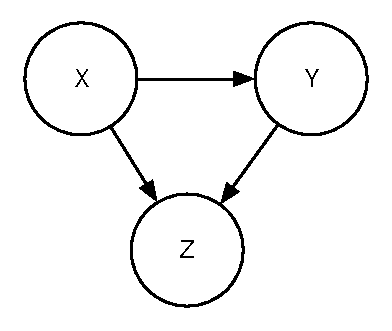
\includegraphics[width=0.4\textwidth]{images/BN.pdf}
\caption{A simple Bayesian network}
\label{fig:bn}
\end{figure}

A dynamic Bayesian network (DBN) is a Bayesian network where the random variables are allowed to depend on prior settings of the same random variables as well as eachother, see figure~\ref{fig:dbn}.

\begin{figure}[H]
    \centering
    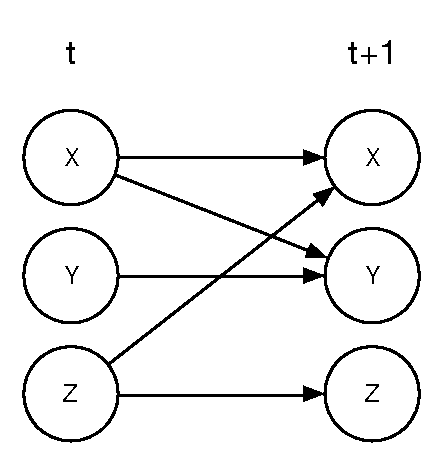
\includegraphics[width=0.5\textwidth]{images/DBN.pdf}
    \caption{A simple dynamic Bayesian network}
    \label{fig:dbn}
\end{figure}

Transition probabilities for the states of an MDP can be represented by a set of Bayesian networks, one network for each possible action. Such a network is comprised of a node, $n_i$, for each state variable, representing that state variable at time $t$, as well as a node, $n_i'$ for each state variable representing the value of that state variable at time $t+1$. If the probability distribution of a certain state variabel $n_k'$ is affected by the value of another state variable $n_j$ if action $a$ is taken then there is a directed edge from $n_j$ to $n_k'$ in the DBN corresponding to action $a$ \parencite{guestrin2003efficient}.
